\documentclass[psamsfonts]{amsart}

%-------Packages---------
\usepackage{amssymb,amsfonts}
\usepackage[all,arc]{xy}
\usepackage{enumerate}
\usepackage[margin=1in]{geometry}
\usepackage{amsthm}
\usepackage{theorem}
\usepackage{verbatim}
\usepackage{tikz}
\usepackage{graphicx}
\usepackage{url}
\usetikzlibrary{shapes,arrows}

\newenvironment{sol}{{\bfseries Solution:}}{\qedsymbol}
\newenvironment{prob}{{\bfseries Problem:}}

\bibliographystyle{plain}

\voffset = -10pt
\headheight = 0pt
\topmargin = -20pt
\textheight = 690pt

%--------Meta Data: Fill in your info------
\title{SE342 \\
Computer Vision\\
Assignment 8 SIFT/SURF}

\author{ChingShing}

\begin{document}

\maketitle

\section{SIFT and SURF Output Files}

\graphicspath{{/Users/ching_shing/Documents/0Junior/Vision/SE342 Computer\ Vision/8\ SIFT/SIFT/}}

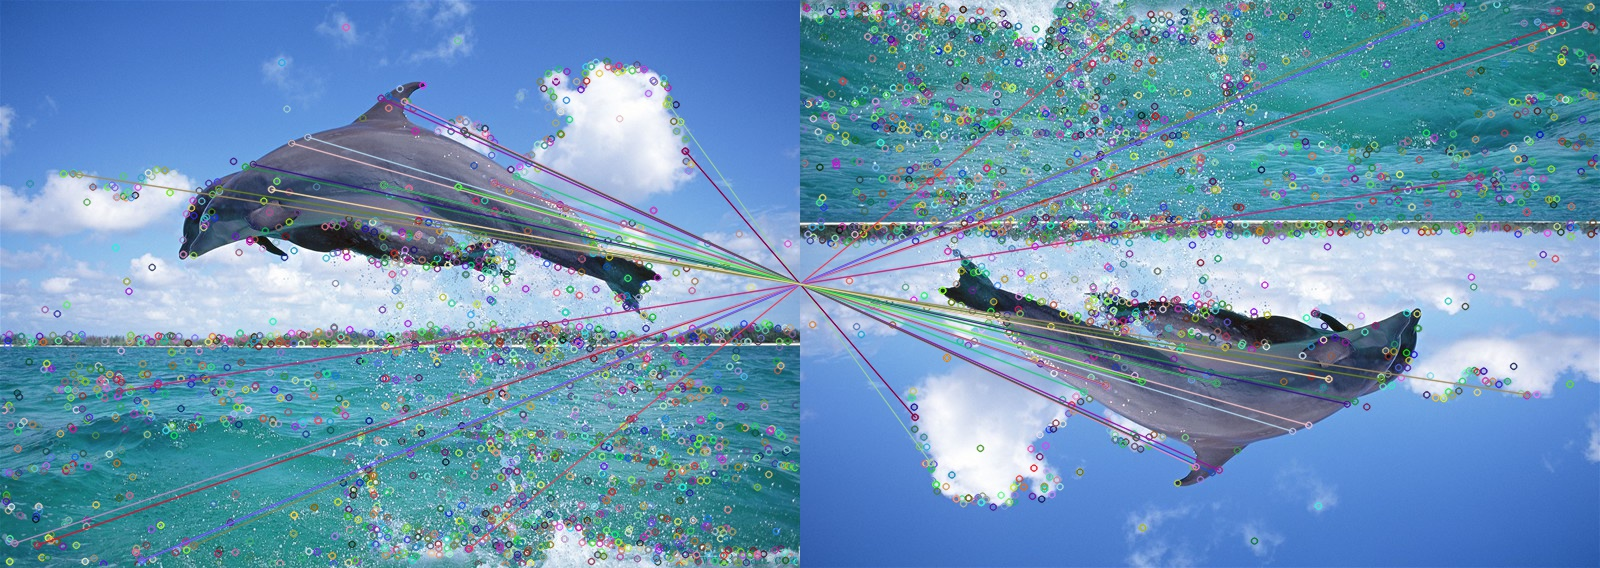
\includegraphics[width=6in]{sift.jpg}

Figure 1. SIFT Output

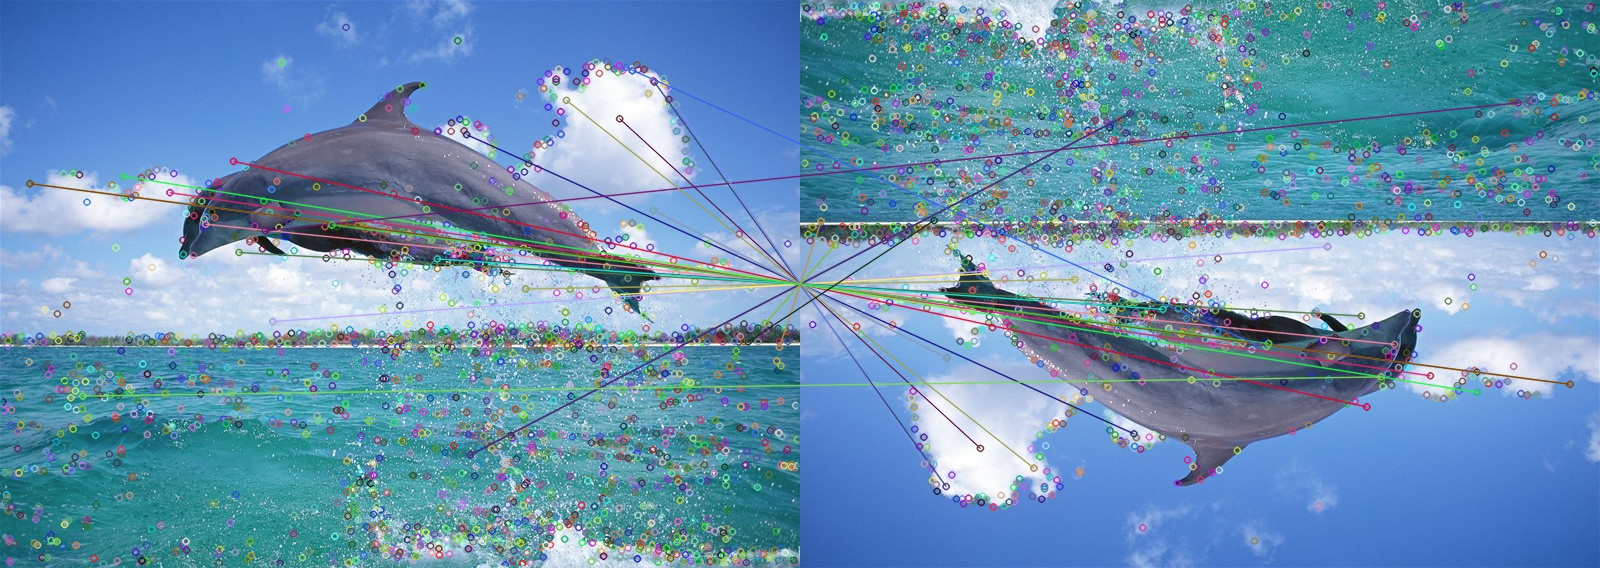
\includegraphics[width=6in]{surf.jpg}

Figure 2. SIRF Output

\section{Algorithm Description}

Algorithm Theory: 
http://opencv-python-tutroals.readthedocs.io/en/latest/py\_tutorials/py\_feature2d/py\_sift

\_intro/py\_sift\_intro.html

1) detect() function finds the keypoint in the images

2) compute() function computes the descriptors from the keypoints we have found

3) match() function matched keypoints between two images by identifying their nearest neighbours

4) only show 30 best-matched keypoints

You can find more detail descriptions in main.cpp

\section{Environment}

Xcode 8.0 with opencv 2.4.13 on Mac OS 10.11

\end{document}
